\documentclass{beamer}
\usetheme{Madrid}
\usecolortheme{whale}
\usepackage{graphicx}
\usepackage{amsmath}

% --- Project Metadata ---
\title[Adaptive Traffic Scheduler]{Adaptive Traffic Light Scheduler}
\subtitle{Comprehensive Project Report: ENR513 Advances in Complex Networks}
\author[Rupani \& Bhati]{Dhairya Rupani, Drumil Bhati}
\institute[Ahmedabad University]{Ahmedabad University}
\date[Winter 2026]{Winter Semester 2026}


\begin{document}

% Slide 1: Title
\begin{frame}
    \titlepage
\end{frame}

% Slide 2: Context & Motivation
\begin{frame}{Context: The Urban Traffic Challenge}
    \begin{itemize}
        \item \textbf{Rapid Urbanization:} Increasing vehicle density leads to unprecedented gridlock in major cities. \pause
        \item \textbf{Economic Impact:} Billions of dollars are lost annually due to fuel waste and reduced productivity. \pause
        \item \textbf{Environmental Cost:} Idle engines at traffic signals significantly contribute to urban air pollution. \pause
        \item \textbf{The Need for Intelligence:} Moving beyond static timers to dynamic, network-aware systems.
    \end{itemize}
\end{frame}

% Slide 3: The Problem Statement
\begin{frame}{The Problem: Limitations of Static Control}
    \begin{itemize}
        \item \textbf{Rigid Timing:} Traditional signals use pre-programmed cycles that ignore real-time demand variations. \pause
        \item \textbf{Isolated Decision Making:} Intersections operate independently, failing to account for neighbor congestion. \pause
        \item \textbf{The "Dead Green" Problem:} Allocating green time to empty lanes while other directions are saturated. \pause
        \item \textbf{Inefficient Resource Allocation:} Static systems cannot prioritize emergency vehicles or high-throughput routes.
    \end{itemize}
\end{frame}

% Slide 4: The Ripple Effect of Congestion
\begin{frame}{Congestion as a Network Phenomenon}
    \begin{columns}
        \begin{column}{0.4\textwidth}
            \begin{itemize}
                \item \textbf{Upstream Propagation:} A single bottleneck can cause queues to spill back. \pause
                \item \textbf{Network Fragility:} Hubs can paralyze the entire city if they fail. \pause
                \item \textbf{Complex Dependencies:} Changing timing affects global traffic patterns.
            \end{itemize}
        \end{column}
        \begin{column}{0.6\textwidth}
            \centering
            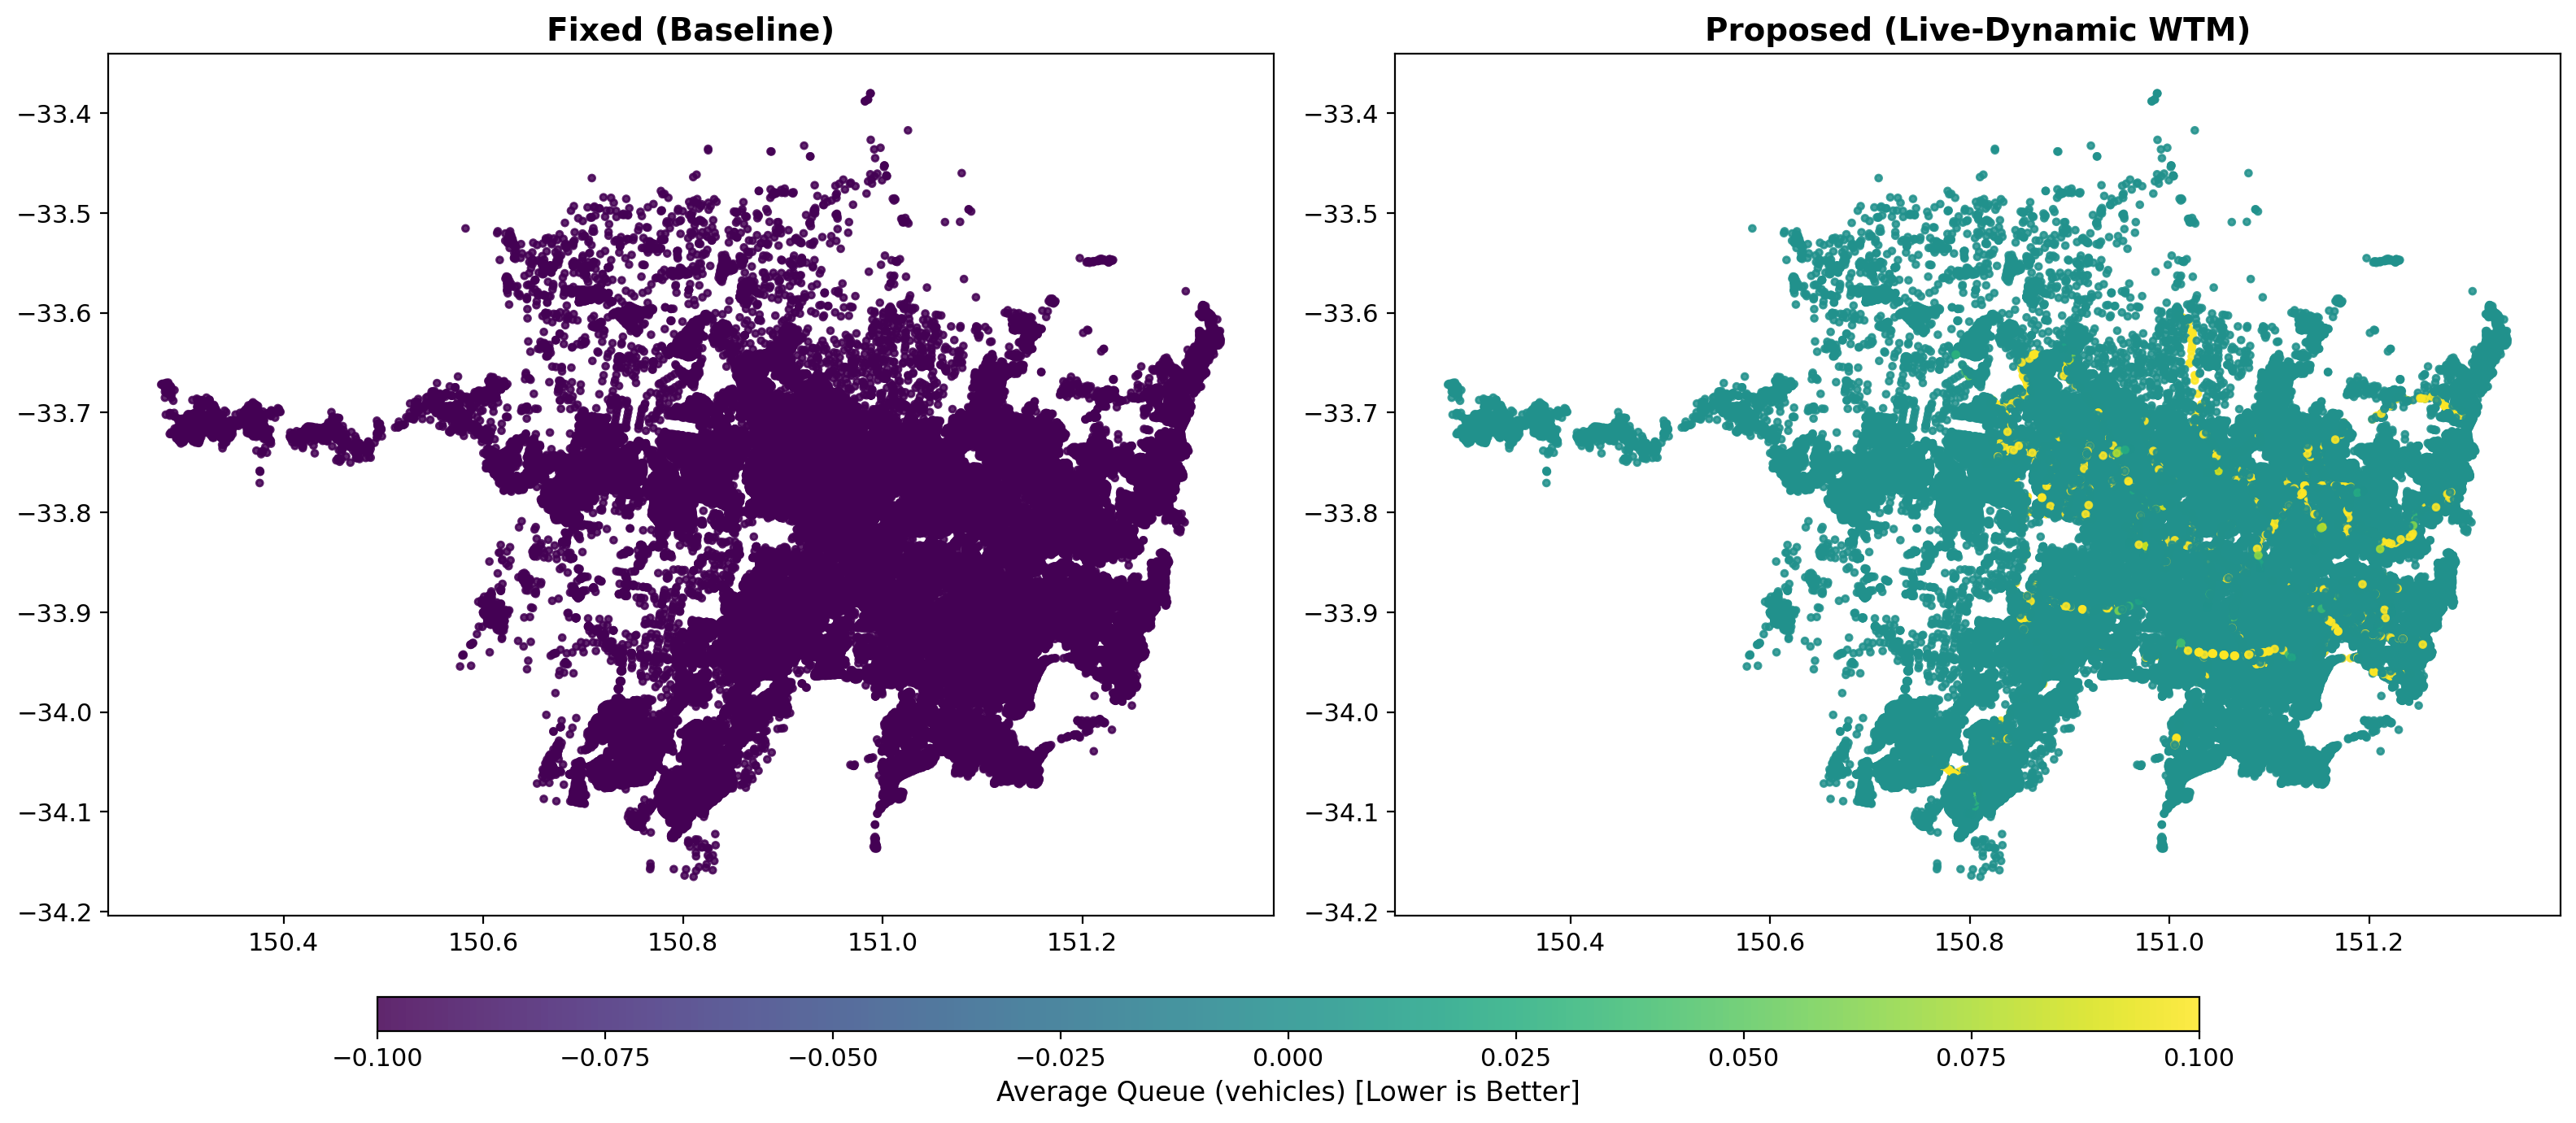
\includegraphics[width=\textwidth]{Sydney/plot5_heatmap_comparison.png} \\
            \tiny{Example Heatmap: Congestion Spreading}
        \end{column}
    \end{columns}
\end{frame}

% Slide 5: Research Objective
\begin{frame}{Research Objective: Weighted Traffic Management}
    \begin{itemize}
        \item \textbf{Goal:} Develop a Live-Dynamic WTM (Weighted Traffic Management) algorithm. \pause
        \item \textbf{Network-Awareness:} Use structural metrics (Centrality) to weight intersection importance. \pause
        \item \textbf{Real-Time Adaptation:} Adjust green light duration based on instantaneous queue lengths and wait times. \pause
        \item \textbf{Benchmarking:} Compare performance against traditional FIXED and BACKPRESSURE controllers.
    \end{itemize}
\end{frame}

% Slide 6: Methodology: City as a Graph
\begin{frame}{Methodology: Modeling the City Network}
    \begin{itemize}
        \item \textbf{Graph Theory Foundation:} Intersections are Nodes ($V$); Roads are directed Edges ($E$). \pause
        \item \textbf{Edge Weights:} Represent road capacity and current occupancy (queues). \pause
        \item \textbf{Dynamic States:} Each node maintains deques of vehicles with arrival timestamps for precise wait-time tracking. \pause
        \item \textbf{Topology Diversity:} Simulations conducted on Nancy, Sydney, Berlin, and Bengaluru layouts.
    \end{itemize}
\end{frame}

% Slide 7: Identifying Important Intersections
\begin{frame}{Structural Importance: Betweenness Centrality}
    \begin{columns}
        \begin{column}{0.4\textwidth}
            \begin{itemize}
                \item \textbf{Definition:} Measures "bridge" nodes on shortest paths. \pause
                \item \textbf{Traffic Role:} Hubs act as global gatekeepers. \pause
                \item \textbf{Gamma Factor ($\gamma$):} Weights the priority score. \pause
                \item \textbf{Proactive Control:} Prioritizing the core.
            \end{itemize}
        \end{column}
        \begin{column}{0.6\textwidth}
            \centering
            \includegraphics[width=0.95\textwidth]{centrality_heatmap.jpeg} \\
            \tiny{Structural Centrality Analysis}
        \end{column}
    \end{columns}
\end{frame}

% Slide 8: The WTM Logic: Scoring System
\begin{frame}{Proposed Solution: The WTM Scoring Algorithm}
    \begin{itemize}
        \item \textbf{Decision Epochs:} At each cycle, the controller evaluates all incoming road segments. \pause
        \item \textbf{Multiplicative Priority:} A situational score determines which direction receives the green light. \pause
        \item \textbf{Fairness vs. Efficiency:} Balancing the need to clear large queues while preventing excessive waits on minor roads. \pause
        \item \textbf{Live Allocation:} The duration of the green phase is scaled proportionally to the winning score.
    \end{itemize}
\end{frame}

% Slide 9: Mathematical Formulation
\begin{frame}{The WTM Score Formula}
    The priority score $S$ for an incoming edge is calculated as:
    \begin{equation*}
        S = (\alpha \cdot P_{queue} + \beta \cdot P_{wait}) \times (1.0 + \gamma \cdot C_{node})
    \end{equation*} \pause
    \begin{itemize}
        \item $\alpha$ (Alpha): Current queue pressure relative to road capacity. \pause
        \item $\beta$ (Beta): Cumulative waiting time of vehicles in the queue. \pause
        \item $\gamma$ (Gamma): Structural importance (Betweenness Centrality) of the source node. \pause
        \item This formula ensures that BOTH local demand and global network importance are weighted.
    \end{itemize}
\end{frame}

% Slide 10: Parameter Tuning: $\alpha$ (Queue Pressure)
\begin{frame}{Parameter Tuning: $\alpha$ (Alpha)}
    \begin{itemize}
        \item \textbf{Role:} Reactive component that responds to physical congestion. \pause
        \item \textbf{Calculation:} Normalized queue length ($L$) divided by Edge Capacity ($C$). \pause
        \item \textbf{Impact:} High $\alpha$ ensures that intersections with long physical lines are prioritized. \pause
        \item \textbf{Dynamic Adjustment:} Nodes with higher in-degrees have higher $\alpha$ sensitivity to manage multi-lane merging.
    \end{itemize}
\end{frame}

% Slide 11: Parameter Tuning: $\beta$ (Wait Time Penalty)
\begin{frame}{Parameter Tuning: $\beta$ (Beta)}
    \begin{itemize}
        \item \textbf{Role:} Fairness component that prevents "starvation" of minor roads. \pause
        \item \textbf{Calculation:} Total cumulative wait time of all vehicles in the current deque. \pause
        \item \textbf{Impact:} Even if a queue is short, if vehicles have been waiting for several cycles, $\beta$ increases their priority. \pause
        \item \textbf{Wait-Sum Logic:} $\sum (T_{current} - T_{arrival})$, ensuring old vehicles have higher weight.
    \end{itemize}
\end{frame}

% Slide 12: Parameter Tuning: $\gamma$ (Structural Weight)
\begin{frame}{Parameter Tuning: $\gamma$ (Gamma)}
    \begin{itemize}
        \item \textbf{Role:} Proactive component that considers network topology. \pause
        \item \textbf{Logic:} Traffic arriving from a central "hub" node is more critical to clear than traffic from a leaf node. \pause
        \item \textbf{Benefit:} Prioritizing flow from central nodes prevents "backlog" from paralyzing the city core. \pause
        \item \textbf{Topological Advantage:} Derived once per network map using NetworkX centrality algorithms.
    \end{itemize}
\end{frame}

% Slide 13: Mapping Topology to Control Parameters
\begin{frame}{Mapping Topology to Control Parameters}
    Graph metrics are normalized and mapped to control sensitivities: \pause
    \begin{itemize}
        \item \textbf{In-Degree ($d$)} $\rightarrow$ \textbf{Alpha ($\alpha$):} $0.5 + 0.5 \cdot \text{norm}(d)$
            \begin{itemize}
                \item High in-degree nodes handle multi-road merging.
                \item $\alpha$ makes them highly reactive to physical queue pressure. \pause
            \end{itemize}
        \item \textbf{Centrality ($c$)} $\rightarrow$ \textbf{Beta ($\beta$):} $0.5 \cdot (1 - \text{norm}(c))$
            \begin{itemize}
                \item Leaf nodes (low $c$) have less frequent traffic.
                \item High $\beta$ ensures these vehicles aren't "starved" by busy hubs. \pause
            \end{itemize}
        \item \textbf{Centrality ($c$)} $\rightarrow$ \textbf{Gamma ($\gamma$):} $0.2 + 0.8 \cdot \text{norm}(c)$
            \begin{itemize}
                \item Hubs (high $c$) are critical for network-wide connectivity.
                \item High $\gamma$ prioritizes clearing the "heart" of the city.
            \end{itemize}
    \end{itemize}
\end{frame}

% Slide 14: Worked Example: 3x3 Grid Parametrization
\begin{frame}{Worked Example: 3x3 Grid Parametrization}
    \begin{center}
        \includegraphics[width=0.45\textwidth]{simulation_snapshot.png} \\
        \tiny{3x3 Grid Topology: Node 4 (Center) vs. Node 0 (Corner)}
    \end{center} \pause
    \begin{itemize}
        \item \textbf{Node 4 (Center Hub):} 
            \begin{itemize}
                \item Centrality: 1.0 $\rightarrow$ $\gamma \approx 1.0$ (Global Priority Hub).
                \item Goal: Keep the network "bridge" open at all costs. \pause
            \end{itemize}
        \item \textbf{Node 0 (Corner Leaf):} 
            \begin{itemize}
                \item Centrality: 0.0 $\rightarrow$ $\gamma \approx 0.2$ (Local Focus).
                \item $\beta \approx 0.5$: Highly sensitive to wait times to maintain fairness. \pause
            \end{itemize}
        \item \textbf{Impact:} The system "knows" its own structure before a single car arrives.
    \end{itemize}
\end{frame}

% Slide 15: Simulation Engine Architecture
\begin{frame}{Implementation: Simulation Architecture}
    \begin{itemize}
        \item \textbf{Discrete Time Simulation:} Vehicles arrive via Poisson distribution at specified rates. \pause
        \item \textbf{Routing:} Shortest-path routing (Dijkstra) dictates vehicle trajectories through the network. \pause
        \item \textbf{State Management:} Deques handle vehicle IDs and timestamps for $O(1)$ arrival/departure logic. \pause
        \item \textbf{Data Collection:} Every step records throughput, wait times, and queue lengths for all nodes.
    \end{itemize}
\end{frame}

% Slide 14: Working Example Walkthrough
\begin{frame}{Walkthrough: 3x3 Grid Working Example}
    \begin{columns}
        \begin{column}{0.4\textwidth}
            \begin{itemize}
                \item \textbf{Step 1: Weighting:} Node 4 (Center) is the hub ($\gamma$). \pause
                \item \textbf{Step 2: Scenarios:}
                    \begin{itemize}
                        \item \textit{Hub:} High $\alpha$ + $\gamma$ = ~45s. \pause
                        \item \textit{Outskirts:} High $\beta$ = ~28s. \pause
                    \end{itemize}
                \item \textbf{Step 3: Reset:} Empty roads default to MIN (15s). \pause
                \item \textbf{Result:} "Heart-first" approach prevents gridlock.
            \end{itemize}
        \end{column}
        \begin{column}{0.6\textwidth}
            \centering
            \includegraphics[width=\textwidth]{simulation_snapshot.png} \\
            \tiny{Simulation: Dynamic Green Light Allocation}
        \end{column}
    \end{columns}
\end{frame}

% Slide 15: Experimental Setup: Multi-City Scope
\begin{frame}{Experimental Setup}
    \begin{itemize}
        \item \textbf{Nancy (France):} High connectivity, medium size. \pause
        \item \textbf{Sydney (Australia):} Large scale, complex topology. \pause
        \item \textbf{Berlin (Germany):} Grid-like patterns with central hubs. \pause
        \item \textbf{Bengaluru (India):} Dense, high-arrival-rate stress testing. \pause
        \item \textbf{Baseline:} Compared against FIXED (60s cycles) and BACKPRESSURE (Max-Weight) controllers.
    \end{itemize}
\end{frame}

% Slide 16: Results: Throughput Analysis
\begin{frame}{Results: Maximizing Throughput}
    \begin{columns}
        \begin{column}{0.4\textwidth}
            \begin{itemize}
                \item \textbf{Nancy:} +93.7\% throughput vs FIXED. \pause
                \item \textbf{Berlin:} 7x more vehicles processed. \pause
                \item \textbf{Efficiency:} Eliminates "starved" green phases.
            \end{itemize}
        \end{column}
        \begin{column}{0.6\textwidth}
            \centering
            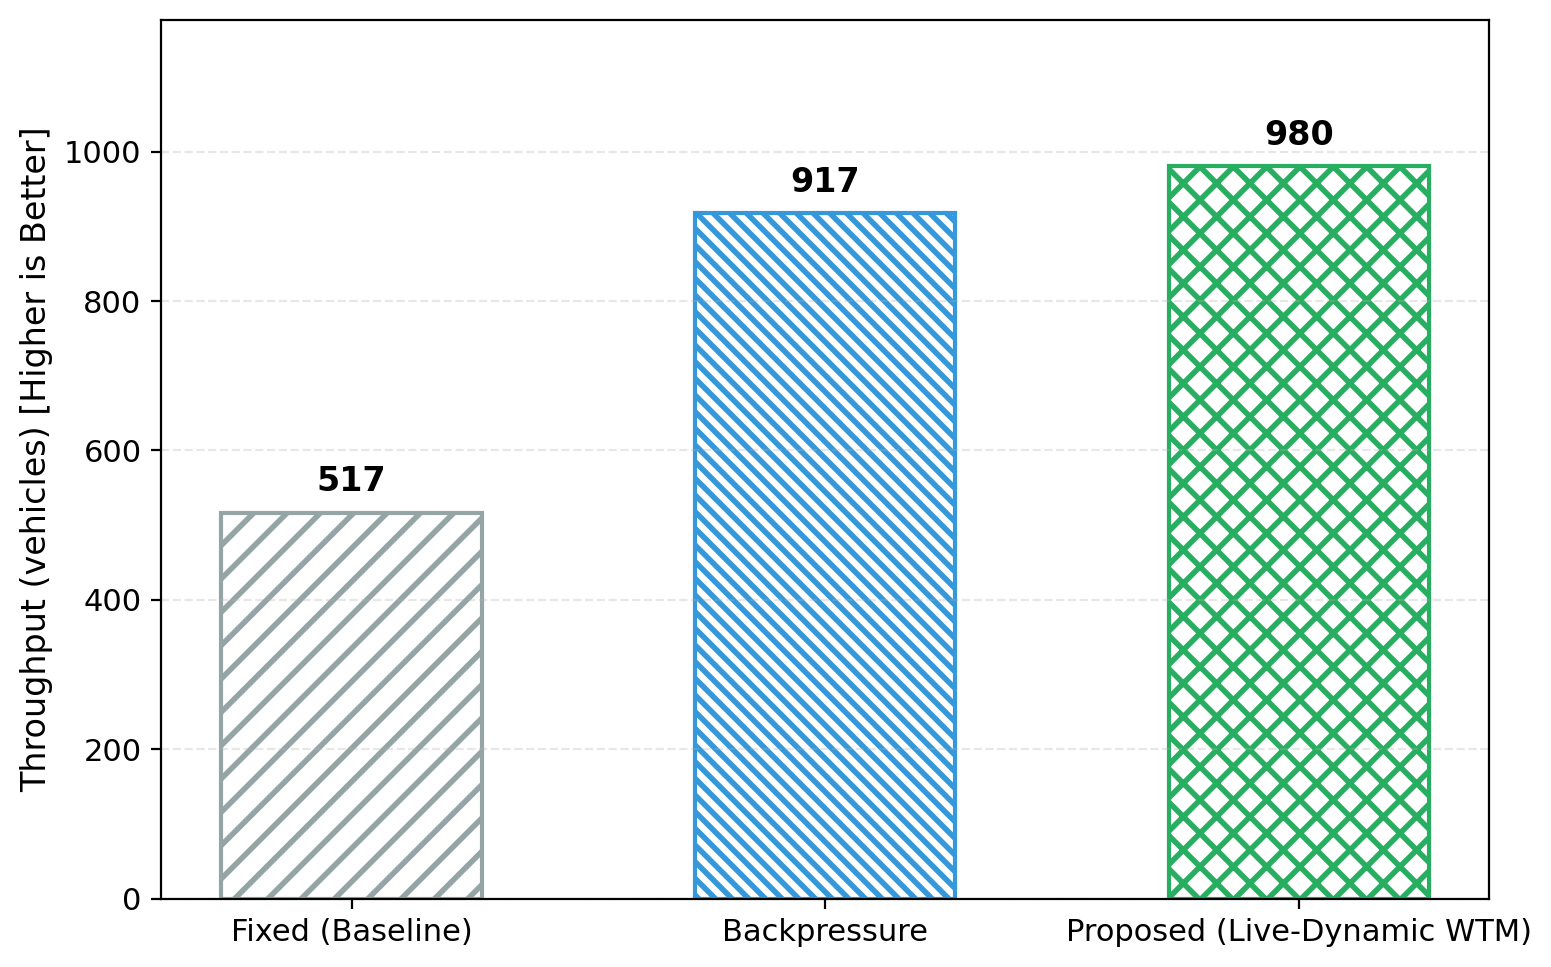
\includegraphics[width=\textwidth]{Nancy/plot3_throughput.png} \\
            \tiny{Throughput Comparison (Nancy)}
        \end{column}
    \end{columns}
\end{frame}

% Slide 17: Results: Wait Time Reduction
\begin{frame}{Results: Minimizing Average Wait Time}
    \begin{columns}
        \begin{column}{0.4\textwidth}
            \begin{itemize}
                \item \textbf{Gains:} Travel time dropped from 2409s to 1895s. \pause
                \item \textbf{Stability:} Consistent 5-10\% lead over Backpressure. \pause
                \item \textbf{Smoothness:} Reduced travel time variance.
            \end{itemize}
        \end{column}
        \begin{column}{0.6\textwidth}
            \centering
            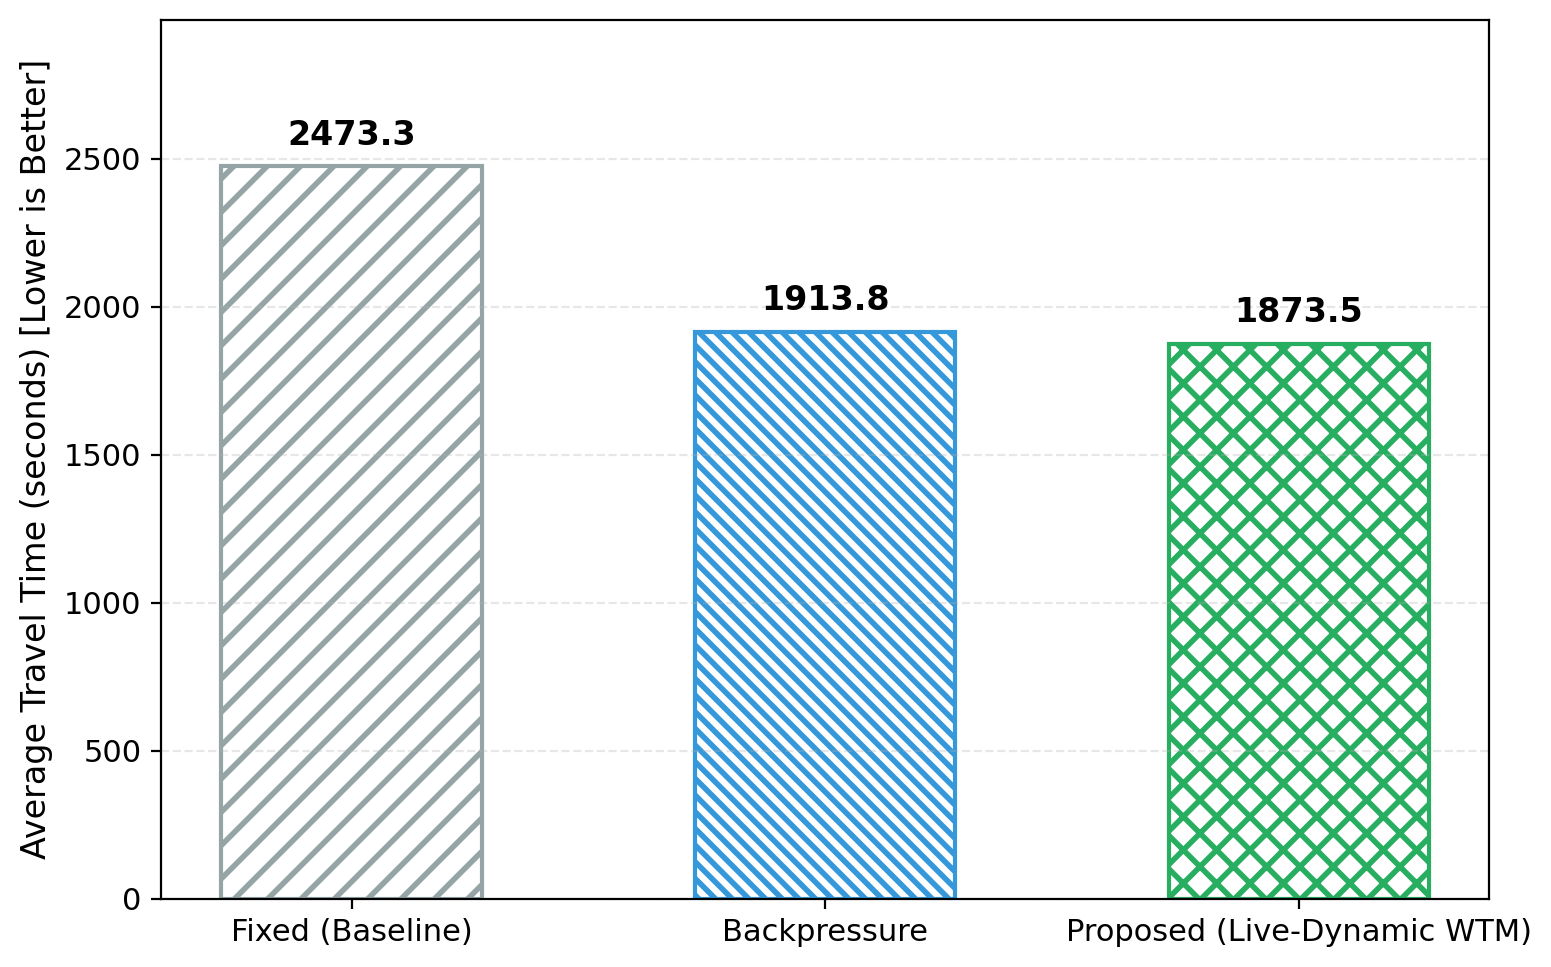
\includegraphics[width=\textwidth]{Nancy/plot2_avg_travel_time.png} \\
            \tiny{Travel Time Reduction}
        \end{column}
    \end{columns}
\end{frame}

% Slide 18: Results: Queue Management
\begin{frame}{Results: Stabilizing Queue Lengths}
    \begin{columns}
        \begin{column}{0.4\textwidth}
            \begin{itemize}
                \item \textbf{Overflow:} Prevents lane spill-back. \pause
                \item \textbf{Gridlock:} Hub prioritization clears core traffic. \pause
                \item \textbf{Damping:} Naturally absorbs traffic surges.
            \end{itemize}
        \end{column}
        \begin{column}{0.6\textwidth}
            \centering
            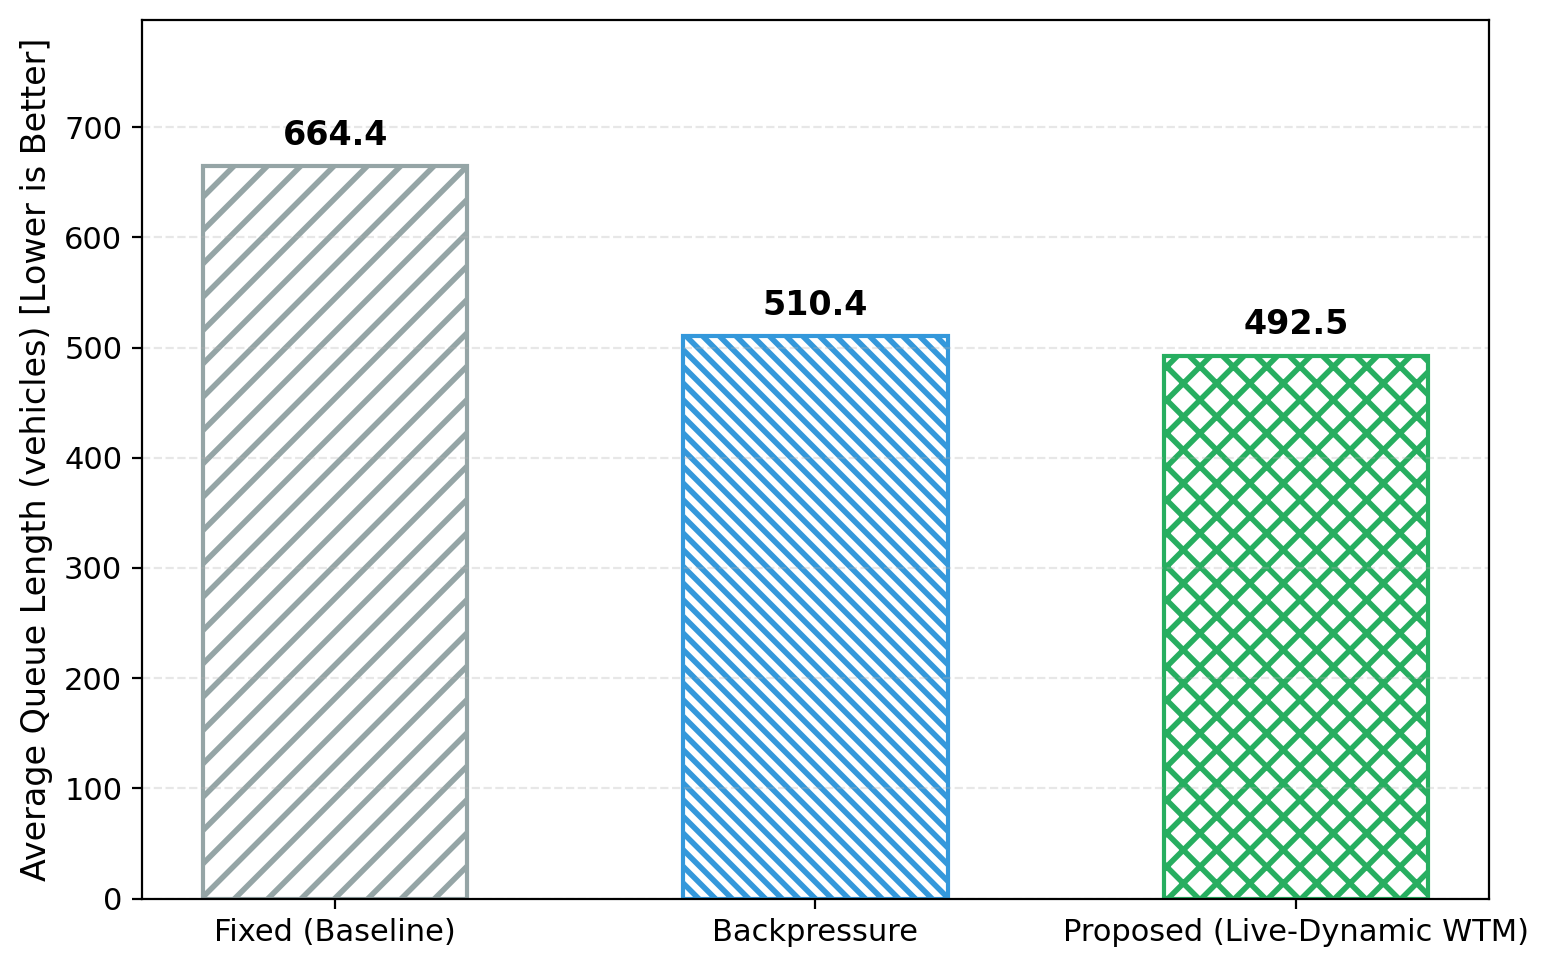
\includegraphics[width=\textwidth]{Nancy/plot1_avg_queue_length.png} \\
            \tiny{Average Queue Stability}
        \end{column}
    \end{columns}
\end{frame}

% Slide 19: Interactive Dashboard & Visualization
\begin{frame}{Project Deliverable: Visual Dashboard}
    \begin{columns}
        \begin{column}{0.4\textwidth}
            \begin{itemize}
                \item \textbf{Real-time:} Color-coded congestion mapping. \pause
                \item \textbf{Interactive:} Toggle between WTM and FIXED. \pause
                \item \textbf{Heatmaps:} Automated bottleneck detection. \pause
                \item \textbf{Stack:} Python, Matplotlib, Folium.
            \end{itemize}
        \end{column}
        \begin{column}{0.6\textwidth}
            \centering
            \includegraphics[width=\textwidth]{dashboard_snapshot.png} \\
            \tiny{Live Animation: Grid Congestion vs. Wait Times}
        \end{column}
    \end{columns}
\end{frame}

% Slide 19: Discussion: Why WTM Wins
\begin{frame}{Discussion: Key Insights}
    \begin{itemize}
        \item \textbf{The Hub Advantage:} Centrality weighting ($\gamma$) is the "secret sauce" that distinguishes WTM from local backpressure. \pause
        \item \textbf{Self-Correction:} The $\beta$ factor ensures that if the system "over-prioritizes" a hub, the side roads eventually get served. \pause
        \item \textbf{Scalability:} The algorithm's local-decision-global-metric approach works regardless of network size.
    \end{itemize}
\end{frame}

% Slide 20: Conclusion & Future Directions
\begin{frame}{Conclusion}
    \begin{itemize}
        \item \textbf{Impact:} Network-aware adaptive scheduling significantly reduces urban congestion. \pause
        \item \textbf{Efficiency:} Live-Dynamic WTM offers up to 90\% higher throughput in high-stress scenarios. \pause
        \item \textbf{Future Work:}
            \begin{itemize}
                \item Integration with Computer Vision (Camera sensors).
                \item Machine Learning to predict future $\alpha, \beta$ trends.
                \item V2I (Vehicle-to-Infrastructure) communication for even finer control.
            \end{itemize}
    \end{itemize}
\end{frame}

% Slide 21: References
\begin{frame}{References}
    \begin{enumerate}
        \item \footnotesize S. Zhang et al., ``A Traffic Graph Convolutional Network for Urban Traffic Prediction,'' \textit{Pattern Recognition}, 2021.
        \item \footnotesize T. Tassmeem et al., ``Backpressure Traffic Signal Control with Network-Wide Weighting,'' \textit{IEEE ITSC}, 2019.
        \item \footnotesize NetworkX Documentation: Centrality Algorithms and Graph Theory.
        \item \footnotesize ResearchGate: Heatmap Analysis for Urban Congestion Patterns.
    \end{enumerate}
\end{frame}

\end{document}
